\documentclass{tufte-handout}

\title{An Example of the Usage of the Tufte-Handout Style\thanks{Inspired by Edward~R. Tufte!}}

\author[The Tufte-LaTeX Developers]{The Tufte-\LaTeX\ Developers}

%\date{28 March 2010} % without \date command, current date is supplied

%\geometry{showframe} % display margins for debugging page layout

\usepackage{graphicx} % allow embedded images
\setkeys{Gin}{width=\linewidth,totalheight=\textheight,keepaspectratio}
\graphicspath{{graphics/}} % set of paths to search for images
\usepackage{amsmath}  % extended mathematics
\usepackage{booktabs} % book-quality tables
\usepackage{units}    % non-stacked fractions and better unit spacing
\usepackage{multicol} % multiple column layout facilities
\usepackage{lipsum}   % filler text
%\usepackage{xcolor}
\usepackage[dvipsnames]{xcolor} % Load the xcolor package with additional color names
\usepackage{hyperref} % Load the hyperref package for links
\usepackage{enumitem}
\usepackage{csquotes}
\usepackage{fancyvrb} % extended verbatim environments
\fvset{fontsize=\normalsize}% default font size for fancy-verbatim environments

% Standardize command font styles and environments
\newcommand{\doccmd}[1]{\texttt{\textbackslash#1}}% command name -- adds backslash automatically
\newcommand{\docopt}[1]{\ensuremath{\langle}\textrm{\textit{#1}}\ensuremath{\rangle}}% optional command argument
\newcommand{\docarg}[1]{\textrm{\textit{#1}}}% (required) command argument
\newcommand{\docenv}[1]{\textsf{#1}}% environment name
\newcommand{\docpkg}[1]{\texttt{#1}}% package name
\newcommand{\doccls}[1]{\texttt{#1}}% document class name
\newcommand{\docclsopt}[1]{\texttt{#1}}% document class option name
\newenvironment{docspec}{\begin{quote}\noindent}{\end{quote}}% command specification environment
\hypersetup{colorlinks}% uncomment this line if you prefer colored hyperlinks (e.g., for onscreen viewing)
\definecolor{midblue}{rgb}{0.2, 0.2, 0.6}
% The `plain' page style is used on chapter opening pages.
% In Tufte's /Beautiful Evidence/ he never puts page numbers at the
% bottom of pages -- the folios are unexpressed.
\fancypagestyle{plain}{
	\fancyhf{} % clear header and footer fields
	% Uncomment the following five lines of code if you want the opening page
	% of the chapter to express the folio in the lower outside corner.
	%\ifthenelse{\boolean{@tufte@twoside}}
	{\fancyfoot[LE,RO]{\thepage}}
	{\fancyfoot[RE,RO]{\thepage}}
}
% Set the in-text footnote mark in the same typeface as the body text itself.
\def\@makefnmark{\hbox{\@textsuperscript{\normalfont\footnotesize\@thefnmark}}}
% Apply the colors to hyperref
\hypersetup{
	colorlinks=true,    % Colors the text of links instead of drawing boxes around them
	urlcolor=cyan,  % Color for \url and \href links to web addresses
	linkcolor=cyan, % Color for internal document links (e.g., table of contents)
	citecolor=cyan, % Color for bibliographic citations
	filecolor=cyan, % Color for links that open local files
}

\setcounter{secnumdepth}{2}
\renewcommand{\thesubsection}{\arabic{section}.\alph{subsection}}

\title{Branching Policy: `Git/Git Flow' Based Versioning}
\author{Patrick TOCA - D\&T CBRE Ltd}
\date{October 14th, 2025 \textsuperscript{(1)}}



\begin{document}
	
	\maketitle  			
	
	\noindent\hrulefill
	\vspace{2pt} \\	
	\marginnote{%
		\begin{minipage}{\marginparwidth}% % Confines the ToC to the margin's width
			\subsection*{Outline of the hand-out}
			\begin{enumerate}
				\item Advantages of the Git/Git Flow based process
				\item General concepts of versioning with Git/Git Flow
				\item Branching terminology and what it implies
				\item Git Flow commands in practice
				\item Conclusion
				\item Useful links
			\end{enumerate}
 
		\end{minipage}%
	}
	This document describes the branching policy of the \enquote{D\&T} team, and presents also how to use it on a day to day basis.\\
	The objectives of this document are:
	\begin{enumerate}[label=\alph*., itemsep=0.2\baselineskip, topsep=0.5\baselineskip, leftmargin=*]
		\item to describe the fundamentals principles of the Git/Git Flow versioning process,
		\item to present the added values presented by this Git/Git Flow based process,
		\item to provide sufficient guidelines to help everyone in the team to get started and become proficient in short time.
	\end{enumerate}
	
	This handout is aimed at the members of the \enquote{D\&T} team(s) and has been distributed before the training session on Git/Git Flow held on January 2019.\\
	\noindent\hrulefill
	\vspace{3pt}

	
	\section{Advantages of the Git/Git Flow Based Process}
	
	Git/Git Flow facilitates the realization of a simple working process within the development team.
	
	It enforces certain practices such as naming conventions for your branches and assists with the flow from development, to release, to master.
	
	Git/Git Flow doesn't offer anything that basic git commands can't do.
	
	With the `start` and `finish` commands Git Flow only abstracts away the merging and deleting Git native commands, a simplification.
	
	\subsection*{Benefits are:}
	\begin{itemize}
		\item enforces a process (flow) by having known branch types: master, develop, feature, release, hotfix
		\item standardises branch naming conventions
		\item abstracts certain git commands for merging and deleting (See link here: Git and \href{https://gist.github.com/JamesMGreene/cdd0ac49f90c987e45ac}{Git Flow commands comparison: a simplification} )
		\item standardises our branching policy on validated practices.
	\end{itemize}

	\footnotetext[1]{first created on 20th December, 2018}
	
	\clearpage
	
	\section{General Concepts of Versioning with Git/Git Flow}
	
	The document: \emph{\href{https://git-scm.com/book/en/v2/Git-Basics-Getting-a-Git-Repository}{Git the essential concepts}} presents in detail what we introduce here.
	
	Git stores and thinks about information in a very different way than other VCS (Subversion, etc.), and understanding these differences will help you avoid becoming confused while using it.
	
	\subsection{Snapshots, Not Differences}
	
	Git thinks of its data more like a series of snapshots of a miniature filesystem. With Git, every time you commit, it saves the state of your project.
	
	To be efficient, if files have not changed, Git doesn't store the file again, just a link to the previous identical file it has already stored. Git thinks about its data more like a stream of snapshots.
	
	It makes Git reconsider almost every aspect of version control that most other systems copied from the previous generation.
	
	Git has been one of the very first fully distributed applications ever delivered in production on a large scale.
	
	
	\noindent\hrulefill
	\vspace{3pt} \\	
	
	\textbf{NEED TO KNOW:} Version Control System provides facilities to model files changing over time and distribute different versions efficiently.
	
	The popular version control system Git provides a powerful Merkle DAG object model that captures changes to a filesystem tree in a distributed-friendly way.

	
	\begin{enumerate}
		\item \textbf{Immutable objects} represent Files (blob), Directories (tree), and Changes (commit).
		\item Objects are \textbf{content-addressed}, by the cryptographic hash of their contents.
		\item \textbf{Links to other objects are embedded}, forming a Merkle DAG. This provides many useful integrity and workflow properties.
		\item Most versioning metadata (branches, tags, etc.) are simply pointer references, and thus inexpensive to create and update.
		\item Version changes only update references or add objects.
		\item Distributing version changes to other users is simply transferring objects and updating remote references.(see nota bene ${}^{2}$)
		\footnotetext[2]{Git is one of the first fully distributed, highly concurrent and scalable applications by design.}
	\end{enumerate}
	
	\vspace{3pt}
	\noindent\hrulefill

	
	\clearpage
	
	\subsection{Nearly All Operations Are Local}
	
	Most operations in Git need only local files and resources to operate; generally no information is needed from another computer on your network. Because you have the entire history of the project right there on your local disk, most operations seem almost instantaneous.
	
	This also means that there is very little you can't do if you're offline or off VPN.
	
	\vspace{3pt}
	\noindent\hrulefill
	\vspace{3pt} \\	
	
	\subsection{Git Has Integrity}
	
	Everything in Git is checksummed before it is stored and is then referred to by that checksum. This means it's impossible to change the contents of any file or directory without Git knowing about it.
	
	This functionality is built into Git at the lowest levels and is integral to its philosophy.
	
	The mechanism that Git uses for this checksumming is called a SHA-1 hash.
	
	A SHA-1 hash looks something like this:
	\begin{verbatim}
		24b9da6552252987aa493b52f8696cd6d3boo373
	\end{verbatim}

	
	In fact, Git stores everything in its database not by file name but by the hash value of its contents.
	
	\vspace{3pt}
	\noindent\hrulefill
	\vspace{3pt} \\	
	
	\subsection{Git Generally Only Adds Data}
	
	When you do actions in Git, nearly all of them only add data to the Git database.
	
	It is hard to get the system to do anything that is not undoable or to make it erase data in any way.
	
	See here: \href{https://git-scm.com/book/en/v2/Git-Basics-Undoing-Things#_undoing}{To go further on Undoing things with Git}.
	
	\vspace{3pt}
	\noindent\hrulefill
	\vspace{3pt} \\	
	
	\clearpage
	
	\subsection{Git Manages 3 States}
	
	Pay attention now! Here is the main thing to remember about Git if you want the rest of your learning process to go smoothly.
	
	Git has three main states that your files can reside in: committed, modified, and staged:
		\begin{itemize}
			\begin{marginfigure}[0.75cm]
				\centering
				\includegraphics[width=1.5\textwidth]{Gitflow_stages.png}
				\caption{The 3 Git stages - Working tree, staging and Git directory}
			\end{marginfigure}
			\item \textbf{Committed} means that the data is safely stored in your local database.
			\item \textbf{Modified} means that you have changed the file but have not committed it to your database yet.
			\item \textbf{Staged} means that you have marked a modified file in its current version to go into your next commit snapshot.
		\end{itemize}
		
		\vspace{3pt}
		\noindent\hrulefill
		\vspace{3pt} \\	
	
	
		\clearpage
		
		\section{Branching terminology and what it implies}
		
		The diagram describes a standard work flow according to 4 policies that Gitflow facili-
		tates:
		
		\begin{enumerate}
			\def\labelenumi{\arabic{enumi}.}
			\item
			the Branching policy: Feature, Develop, Release, Hofixes (if any),
			Master
			\item
			the Testing policy: developers can manage features and develop, the QA
			manage Release and the Owner manage Master.
			\item
			the DB policy: a DB and its necessary and sufficient data, for each
			type of testing,
			\item
			the Deployment policy: which environment with which Owner and which
			purpose.
		\end{enumerate}
		
		\begin{figure}	
			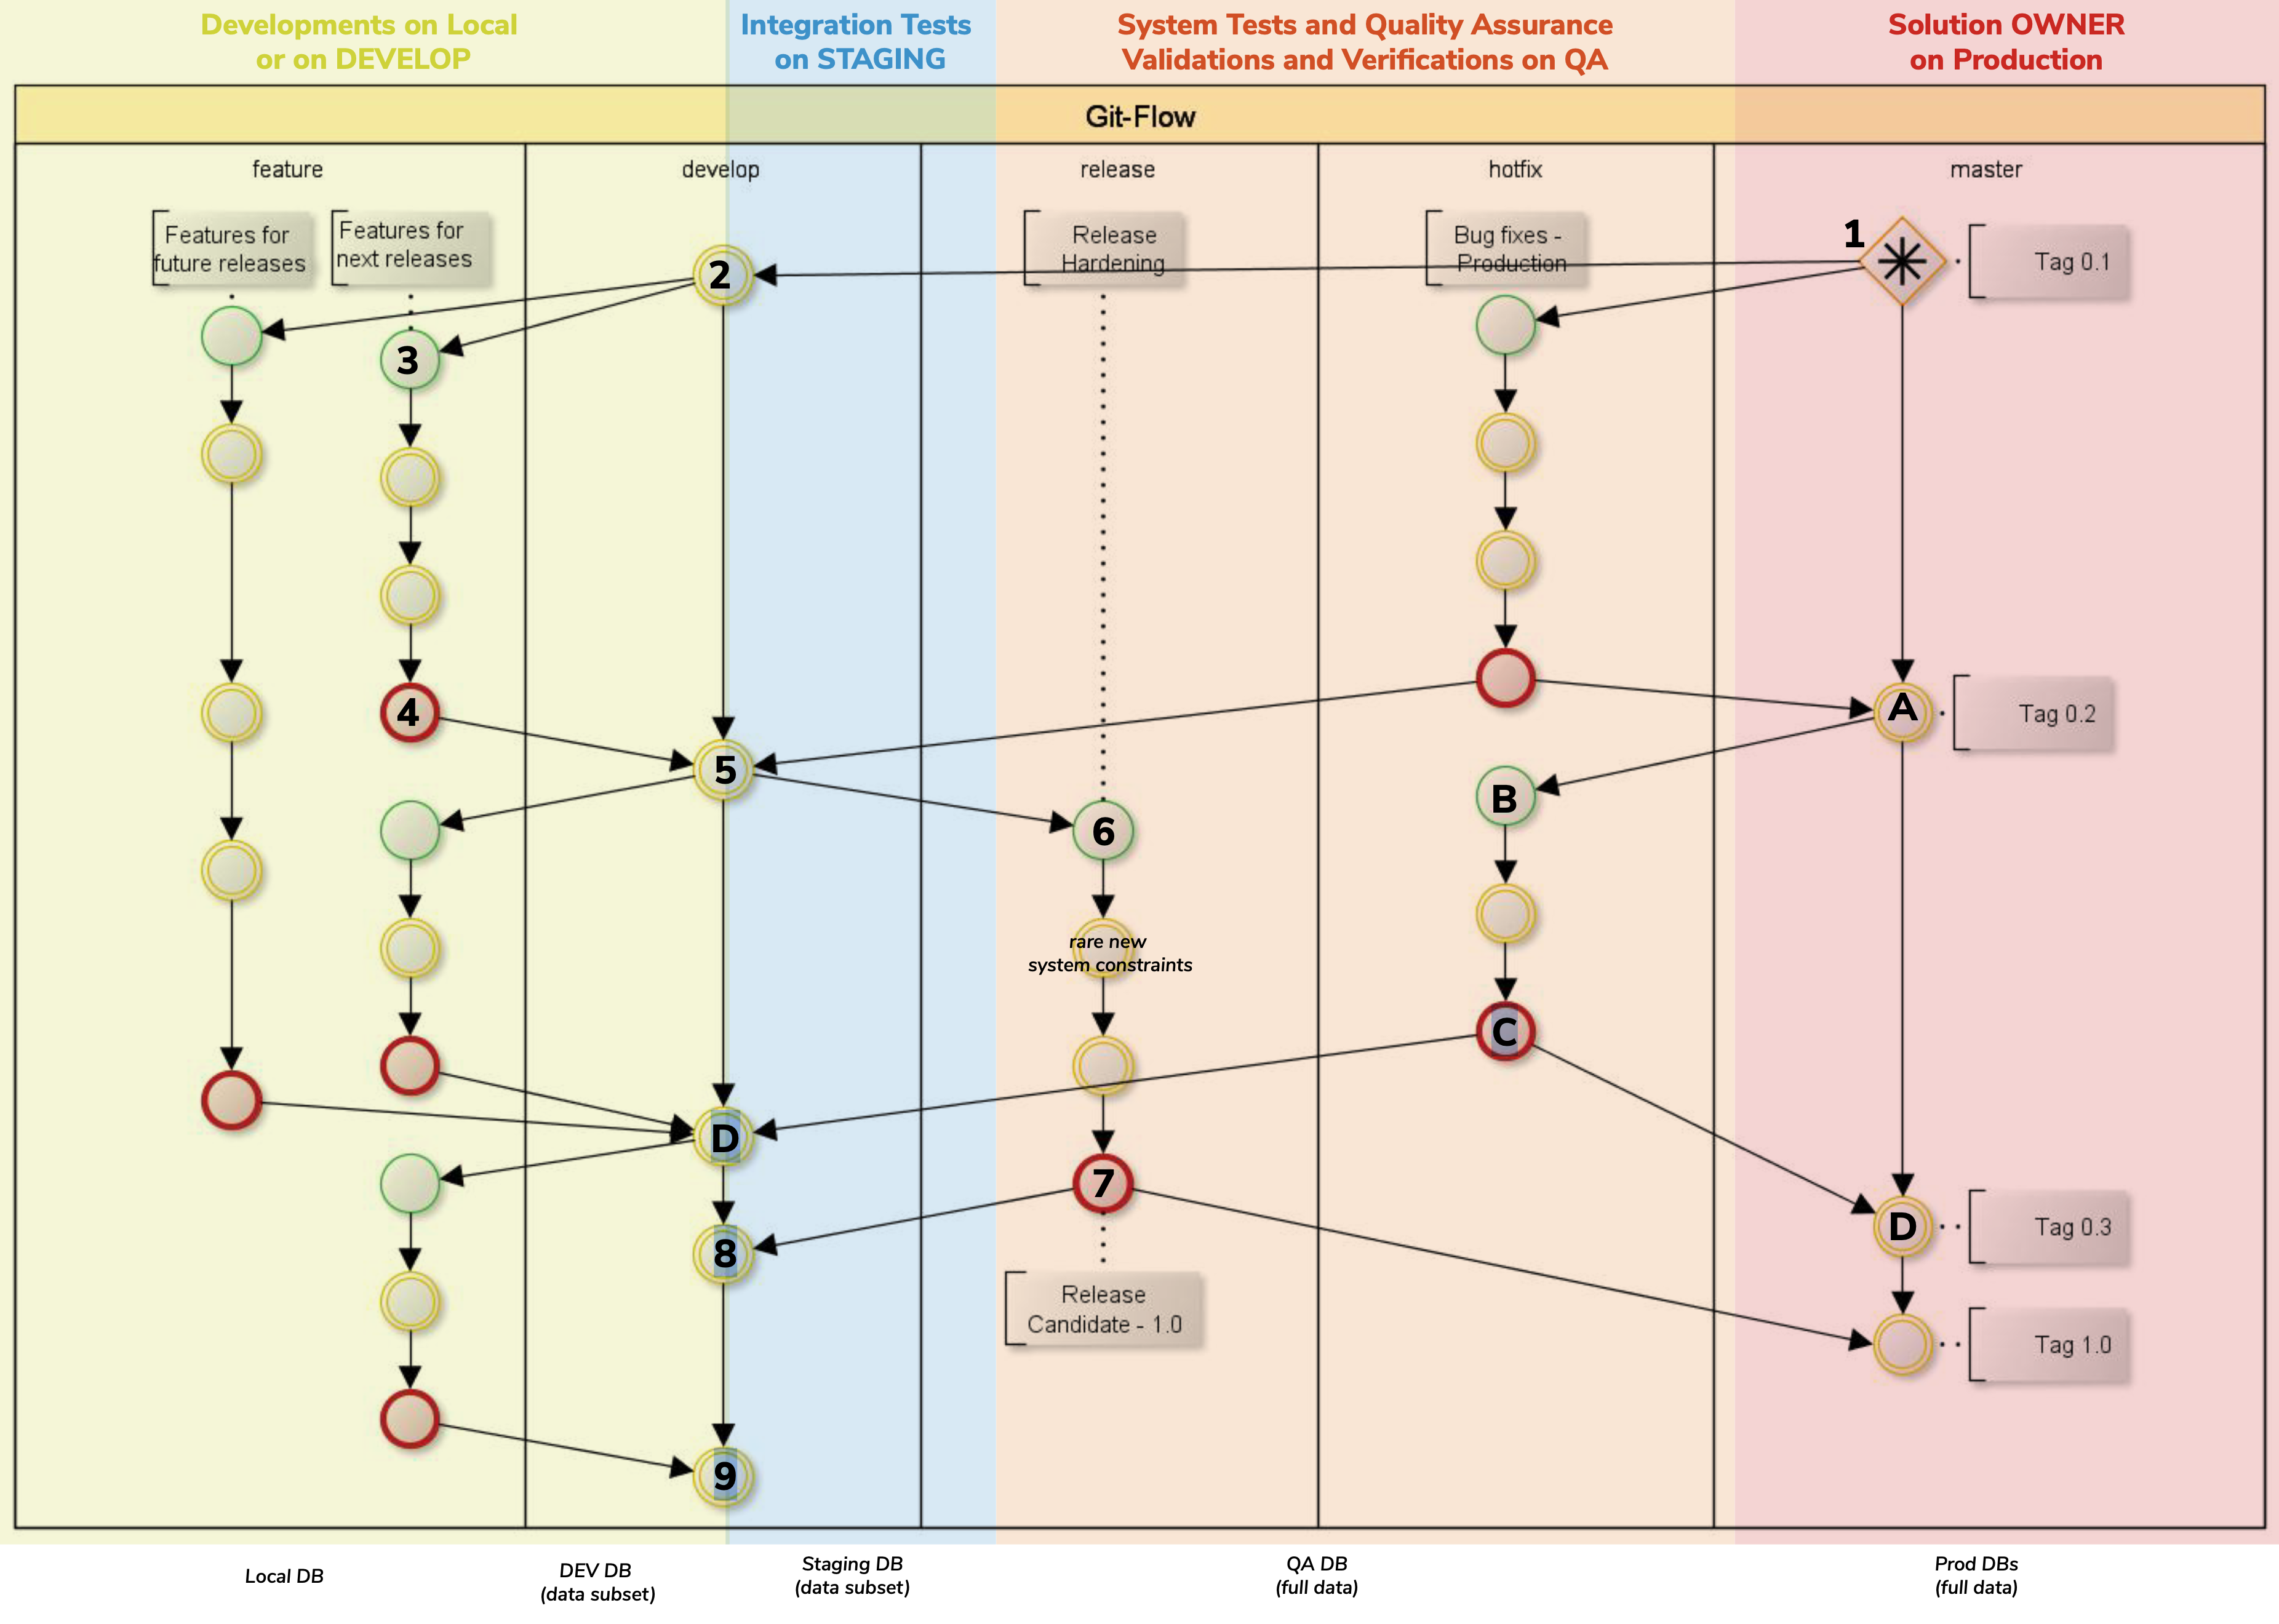
\includegraphics{gitflow_deployment_policy.png}
			%  \checkparity This is an \pageparity\ page.%
			\caption{Branching, Testing. Deployment and DB access policies \\ 
				$\rightarrow$
				\emph{from Master to Develop to Feature and back.}}
			\label{fig:textfig}
			%\zsavepos{pos:textfig}
			%\setfloatalignment{b}
		\end{figure}
		
		
		
		\clearpage
		
		
		\section{\textbf{Gitflow commands in practice}}
		
		
			
		Gitflow simplifies the Git versioning branching process to a few set of
		operations (see nota bene \sidenote{Nota Bene: Using the 'showcommands' switch and Hotfix. you can see the actual git commands being executed by the Gitflow plugin : \textbf{\textcolor{blue}{git flow feature start FEATURE-NAME --showcommands}} }) : Initialise, Connect, Features, Releases\\ 

		\vspace{0.05cm}
		

		\subsection{Initialise}
		
		\begin{table}[ht]
			\centering
			\fontfamily{ppl}\selectfont
			\begin{tabular}{ll}
				%\toprule
				Gitflow & Git \\
				\midrule
				git flow init & git init \\
				 & git commit –allow-empty -m "Initial commit" \\
				 & git checkout -b develop master \\
				%\bottomrule
			\end{tabular}
			\caption{\textcolor{gray}{Git Flow reduces significantly the number of commands}.}
			\label{tab:normaltab}
			\setfloatalignment{b}
		\end{table}
		\medskip % Adds a medium space after the table
		
		\vspace{0.25cm}
		git flow init also edits your .git/config and prompts for values:\\ 		\vspace{0.25cm}		
		\textbf{{[}gitflow ``branch''{]}}
			\begin{itemize}
				\item \small{master = master}
				\item \small{develop = develop}
			\end{itemize}
				\textbf{{[}gitflow ``prefix''{]}} 
			\begin{itemize}
				\item \small{feature = feature}
				\item \small{release = release}
				\item \small{hotfix = hotfix}
				\item \small{support = support}
				\item \small{versiontag = }
			\end{itemize}
	

		\subsection{Connect to Remote repository}
		
		\begin{table}[ht]
			\centering
			\fontfamily{ppl}\selectfont
			\begin{tabular}{ll}
				%\toprule
				Gitflow & Git \\
				\midrule
				git flow init & git init \\
				\textbf{\textcolor{gray}{Already done during the init}} & git remote add origin \\
				& git@github.com:MYACCOUNT/MYREPO \\
				%\bottomrule
			\end{tabular}
			\label{tab:normaltab}
		\end{table}
		\medskip % Adds a medium space after the table
		
		\clearpage
		

		\subsection{Features branching}
		
		\hspace{1em}\textbf{\textcolor{blue}{Creating a feature branch}}
		
		\begin{table}[ht]
			\centering
			\fontfamily{ppl}\selectfont
			\begin{tabular}{ll}
				%\toprule
				Gitflow & Git \\
				\midrule
				git flow feature start MYFEATURE & git checkout -b feature/MYFEATURE develop \\
				%\bottomrule
			\end{tabular}
			\label{tab:normaltab}
		\end{table}
		\medskip % Adds a medium space after the table
		
	    \textbf{\textcolor{blue}{Sharing a feature branch}}
		
		\begin{table}[ht]
			\centering
			\fontfamily{ppl}\selectfont
			\begin{tabular}{ll}
				%\toprule
				Gitflow & Git \\
				\midrule
				git flow feature publish MYFEATURE & git checkout feature/MYFEATURE \\
				& git push origin feature/MYFEATURE \\
				%\bottomrule
			\end{tabular}
			\label{tab:normaltab}
		\end{table}
		\medskip % Adds a medium space after the table
		
		\textbf{\textcolor{blue}{Get latest for a feature branch}}
		
		\begin{table}[ht]
			\centering
			\fontfamily{ppl}\selectfont
			\begin{tabular}{ll}
				%\toprule
				Gitflow & Git \\
				\midrule
				git flow feature pull origin MYFEATURE & git init \\
				& git checkout feature/MYFEATURE \\
				& git pull --rebase origin feature/MYFEATURE \\
				%\bottomrule
			\end{tabular}
			\label{tab:normaltab}
		\end{table}
		\medskip % Adds a medium space after the table
		
				
		\clearpage

		\textbf{\textcolor{blue}{Finalize a feature branch}}
		
		\begin{table}[ht]
			\centering
			\fontfamily{ppl}\selectfont
			\begin{tabular}{ll}
				%\toprule
				Gitflow & Git \\
				\midrule
				git flow feature finish MYFEATUR & git checkout develop \\
				& git merge --no-ff feature/MYFEATURE \\
				& git branch -d feature/MYFEATURE \\
				%\bottomrule
			\end{tabular}
			\label{tab:normaltab}
		\end{table}
		\medskip % Adds a medium space after the table
		
		
		\textbf{\textcolor{blue}{Push the merged feature branch}}
		
		\begin{table}[ht]
			\centering
			\fontfamily{ppl}\selectfont
			\begin{tabular}{ll}
				%\toprule
				Gitflow & Git \\
				\midrule
				\textbf{\textcolor{gray}{Already done during the finish}} & git push origin develop \\
				& git push origin :feature/MYFEATURE (if pushed) \\
				%\bottomrule
			\end{tabular}
			\label{tab:normaltab}
		\end{table}
		\medskip % Adds a medium space after the table
		
		\clearpage
		
		\subsection{Releases branching}
		
		\hspace{1em}\textbf{\textcolor{blue}{Create a release branch}}
		
		\begin{table}[ht]
			\centering
			\fontfamily{ppl}\selectfont
			\begin{tabular}{ll}
				%\toprule
				Gitflow & Git \\
				\midrule
				git flow release start \textbf{\textcolor{gray}{v1.2.0}} & git checkout -b release/v1.2.0 develop \\
				%\bottomrule
			\end{tabular}
			\label{tab:normaltab}
		\end{table}
		\medskip % Adds a medium space after the table
		

		\textbf{\textcolor{blue}{Share a release branch}}
		
		\begin{table}[ht]
			\centering
			\fontfamily{ppl}\selectfont
			\begin{tabular}{ll}
				%\toprule
				Gitflow & Git \\
				\midrule
				git flow release publish \textbf{\textcolor{gray}{v1.2.0}} & git checkout -b
				\textbf{\textcolor{gray}{release/v1.2.0}} develop \\
				%\bottomrule
			\end{tabular}
			\label{tab:normaltab}
		\end{table}
		\medskip % Adds a medium space after the table


		\textbf{\textcolor{blue}{Get latest for a release branch}}
		
		\begin{table}[ht]
			\centering
			\fontfamily{ppl}\selectfont
			\begin{tabular}{ll}
				%\toprule
				Gitflow & Git \\
				\midrule
				\textbf{\textcolor{gray}{Already done during the finish}} & git checkout -b \textbf{\textcolor{gray}{release/v1.2.0}} develop \\
				& git pull --rebase origin \textbf{\textcolor{gray}{release/v1.2.0}} \\
				%\bottomrule
			\end{tabular}
			\label{tab:normaltab}
		\end{table}
		\medskip % Adds a medium space after the table
		
	 	\clearpage

		\textbf{\textcolor{blue}{Finalize a release branch}}
		
		\begin{table}[ht]
			\centering
			\fontfamily{ppl}\selectfont
			\begin{tabular}{ll}
				%\toprule
				Gitflow & Git \\
				\midrule
				git flow release finish \textbf{\textcolor{gray}{v1.2.0}} & git checkout master \\
				& git pull --rebase origin \textbf{\textcolor{gray}{release/v1.2.0}} \\
				& git merge --no-ff \textbf{\textcolor{gray}{release/v1.2.0}} \\
				& git tag -a \textbf{\textcolor{gray}{v1.2.0}} \$RELEASE\_BRANCH (to include the branch name) \\
				& git checkout develop \\
				& git merge --no-ff \textbf{\textcolor{gray}{release/v1.2.0}} \\
				& git branch -d \textbf{\textcolor{gray}{release/v1.2.0}} \\ 
				%\bottomrule
			\end{tabular}
			\label{tab:normaltab}
		\end{table}
		\medskip % Adds a medium space after the table
		

		\textbf{\textcolor{blue}{Push the merged release branch}}
		
		\begin{table}[ht]
			\centering
			\fontfamily{ppl}\selectfont
			\begin{tabular}{ll}
				%\toprule
				Gitflow & Git \\
				\midrule
				\textbf{\textcolor{gray}{Already done during the finish}} & git push origin master \\
				& git push origin develop \\
				& git push origin --tags \\
				& git push origin:\textbf{\textcolor{gray}{release/v1.2.0}} (if pushed) \\
				%\bottomrule
			\end{tabular}
			\label{tab:normaltab}
		\end{table}
		\medskip % Adds a medium space after the table
		
		\clearpage
		

		\subsection{Hotfixes branching}
		
		\hspace{1em}\textbf{\textcolor{blue}{Create a hotfix branch}}
		
		\begin{table}[ht]
			\centering
			\fontfamily{ppl}\selectfont
			\begin{tabular}{ll}
				%\toprule
				Gitflow & Git \\
				\midrule
				git flow hotfix start \textbf{\textcolor{gray}{v1.2.1}} {[}commit{]} & git checkout -b \textbf{\textcolor{gray}{hotfix/v1.2.1}} {[}commit{]} \\
				%\bottomrule
			\end{tabular}
			\label{tab:normaltab}
		\end{table}
		\medskip % Adds a medium space after the table
		
		
		\textbf{\textcolor{blue}{Finalize a hotfix branch}}
	
		
		\begin{table}[ht]
			\centering
			\fontfamily{ppl}\selectfont
			\begin{tabular}{ll}
				%\toprule
				Gitflow & Git \\
				\midrule
				git flow hotfix finish \textbf{\textcolor{gray}{v1.2.1}} & git checkout master \\
				& git merge --no-ff \textbf{\textcolor{gray}{hotfix/v1.2.1}} \\
				& git tag -a \textbf{\textcolor{gray}{v1.2.1}} \\
				& git checkout develop \\
				& git merge --no-ff \textbf{\textcolor{gray}{hotfix/v1.2.1}} \\
				& git branch -d \textbf{\textcolor{gray}{hotfix/v1.2.1}} \\
				%\bottomrule
			\end{tabular}
			\label{tab:normaltab}
		\end{table}
		\medskip % Adds a medium space after the table	
		
		\textbf{\textcolor{blue}{Push the merged hotfix branch}}
		
		\begin{table}[ht]
			\centering
			\fontfamily{ppl}\selectfont
			\begin{tabular}{ll}
				%\toprule
				Gitflow & Git \\
				\midrule
				\textbf{\textcolor{gray}{Already done during the finish}} & git push origin master \\
				& git push origin develop \\
				& git push origin --tags \\
				& git push origin:\textbf{\textcolor{gray}{hotfix/v1.2.1}} (if pushed) \\
				%\bottomrule
			\end{tabular}
			\label{tab:normaltab}
		\end{table}
		\medskip % Adds a medium space after the table
		
		\clearpage
		
		
		
		\section{Conclusion}
	
		
		Git-Flow is an extremely powerful workflow for doing development and
		seems to cater for just about every scenario you can come across in
		business. It is simple to follow once you start using it and makes for a
		good standard across small and big companies. If you use it in
		conjunction with Git you'll quickly realize the strength of it (combined
		with Test Driven Development practices, Continuous Integration as well
		as Regression Testing scenarios) while not even taking into
		consideration the usual effort that goes into doing a Release or even a
		Hotfix.
		\bigskip
		
		\textbf{\textcolor{gray}{Parallel Development}}\\
		One of the great things about GitFlow is that it makes parallel de- velopment very easy, by isolating new development from finished work. New development (such as features and non-emergency bug fixes) is done in feature branches, and is only merged back into main body of code when the developer(s) is happy that the code is ready for release. Although interruptions are a BadThing(tm), if you are asked to switch from one task to another, all you need to do is commit your changes and then create a new feature branch for your new task. When that task is done, just checkout you r original feature branch and you can continue where you left off.
		\medskip
		
		\textbf{\textcolor{gray}{Collaboration Feature}}\\
		Branches also make it easier for two or more
		developers to collaborate on the same feature, because each feature
		branch is a sandbox where the only changes are the changes necessary to get the new
		feature working. That makes it very easy to see and follow what each
		collaborator is doing.
		\medskip
		
		\textbf{\textcolor{gray}{Release Staging Area}}\\
		As new development is completed, it gets merged
		back into the de- velop branch, which is a staging area for all
		completed features that haven't yet been released. So when the next
		release is branched off of develop, it will auto- matically contain all
		of the new stuff that has been finished.
		\medskip
		
		\textbf{\textcolor{gray}{Support For Emergency Fixes}}\\
		GitFlow supports hotfix branches -
		branches made from a tagged release. You can use these to make an
		emergency change, safe in the knowledge that the hotfix will only
		contain your emergency fix. There's no risk that you'll accidentally
		merge in new development at the same time.
		
		\clearpage
		
		\subsection{Useful links}
		
		\begin{enumerate}
			\def\labelenumi{\arabic{enumi}.}
			\item
			\href{https://danielkummer.github.io/git-flow-cheatsheet/#features}{a graphic representation 0f the Gitflow process}
			\item
			\href{https://nvie.com/posts/a-successful-git-branching-model/}{Vincent Driessen's original blog post about Gitflow - 2010}
			\item
			\href{https://datasift.github.io/gitflow/GitFlowForGitHub.html}{Gitflow for Github: further consolidation}
			\item
			\href{https://veerasundar.com/blog/2018/03/gitflow-animated/}{Gitflow animation}
			\item
			\href{https://github.com/nvie/gitflow/}{Finally, to install Gitflow on your laptop}
		\end{enumerate}
	
\end{document}